\chapter{Analysis of the pattern recognition problem}
\label{ch:Analysis of the pattern recognition problem}

\section{Analysis of the time series data}
\label{sec:Analysis of the time series data}
This chapter will provide a closer examination of the time series data measured by the Texas Intrument's SensorTag. This data is prerequisite for the further work of this paper. \newline
The sensor data is measured and collected at a sampling rate of 10 measurements per second. To optimize accuracy, the maximal sampeling rate of the Texas Instrument's SensorTag was chosen.  The measurements include acceleration in 3 spacial axis. The axis each correspond to a direction on the Sensorboard and are orthogonal to each other as shown in figure \ref{fig:xyzboard}. The acceleration is measured in g, which refers to the acceleration that is imparted by the gravity of earth. For g the following convertion to  $m/s^2 $ holds true: $ 1 g = 9.80665 m/s^2 $. 
\\
The acceleration in any particular direction will be referred to as x, y or z acceleration.

\begin{figure}[h]
\centering
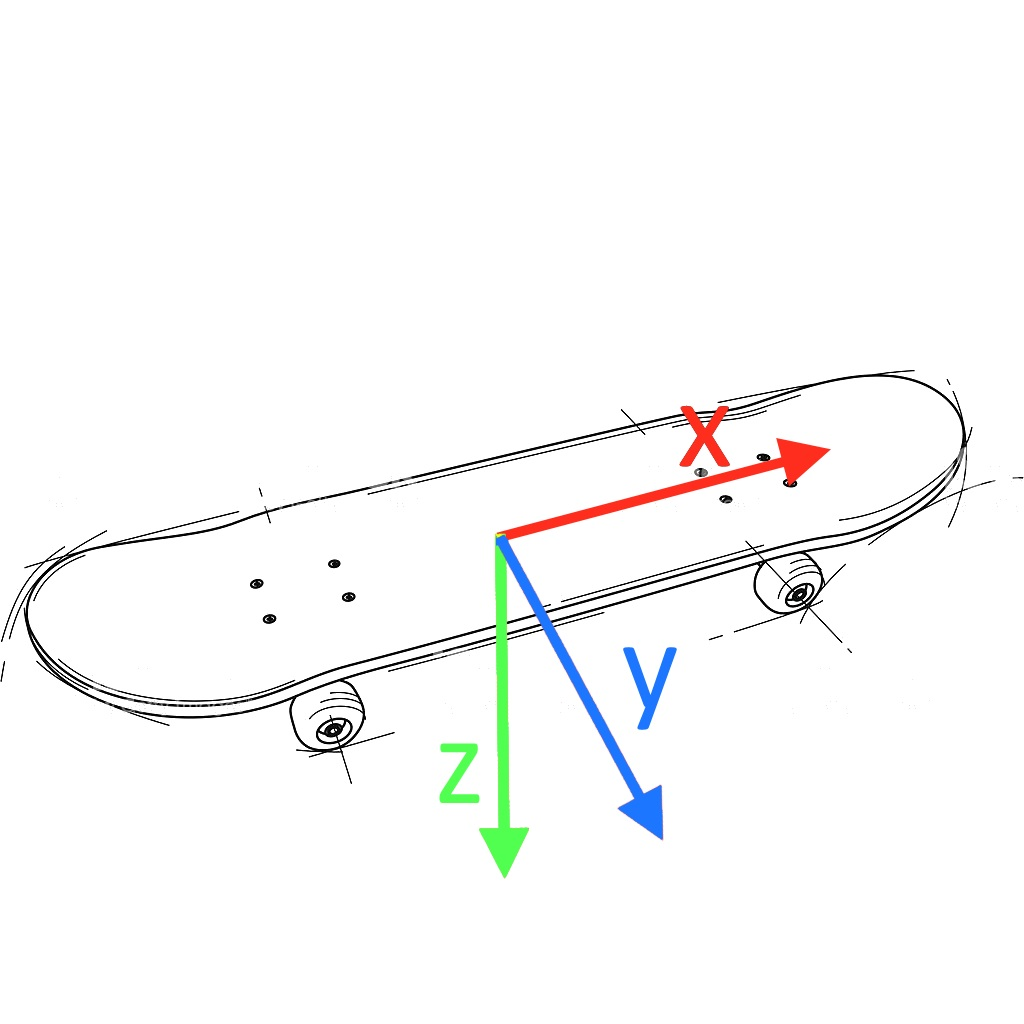
\includegraphics[width=0.7\textwidth]{PE4/xyz.JPG}
\caption{Illustration of Sensorboard and axis of measurement. The driving direction is to the right.}
\label{fig:xyzboard}
\end{figure}


The measurements are taken  simultaneously and handled together as one measurement collection. This collection is enriched with the time of the measurement  in form of a Unix timestamp.\\
A measurement collection as described above will also be referred to as a data point. The single measurements (for instance x acceleration) of a measurement collection are the features of a data point.\\
An exemplary data point in a key-value-pair format can be seen here in figure \ref{fig:datapointjson}.
\begin{figure}[h]
\centering
\begin{lstlisting}
{
  "accx": -0.079590,
  "accy": 0.001465,
  "accz": -1.016602,
  "time": 1502735960911
}
\end{lstlisting}
\caption{Example data point in key-value-pair notation notation}
\label{fig:datapointjson}
\end{figure}
The keys in figure \ref{fig:datapointjson} stand for acceleration in x direction, acceleration in y direction, acceleration in z direction and the Unix timestamp when the measurement took place. \\
Using the time of measurement, data can be plotted on a time axis plot as seen in figure \ref{fig:timeaxis}.


\begin{figure}[h]
\centering
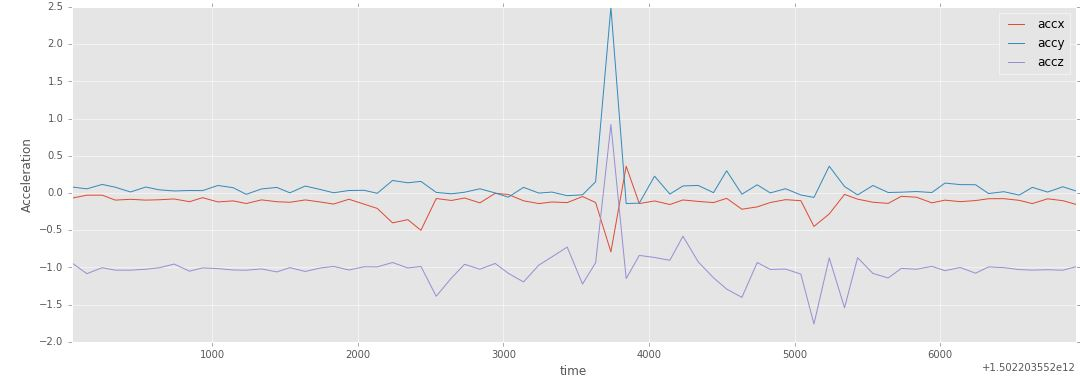
\includegraphics[width=0.9\textwidth]{PE4/timeseriesdata.JPG}
\caption{Example of measured accelerations on 3 Axis during a collision }
\label{fig:timeaxis}
\end{figure}

Data from the Sensorboard has been collected in isolated experiments. During the experiments of the Sensorboard 69 collisions were simulated. Accordingly, 69 of the 6453 data points collected,  were labelled as a collision while the rest was labelled  as no collision. The labelling was implemented by analysing video footage, recorded during the experiment. The exact time of a collision in the video was matched with the time of the recorded sensor data to label data points correctly.\\
The distribution of the data points labeled as collision or no collision can be seen in figure \ref{fig:xyscatter}. The scatter plot shows the relationship between the x and z acceleration and the label of the data point. The y acceleration is not visualized here. A blue data point represent a collision the red data points represent no collision.

\begin{figure}[h]
\centering
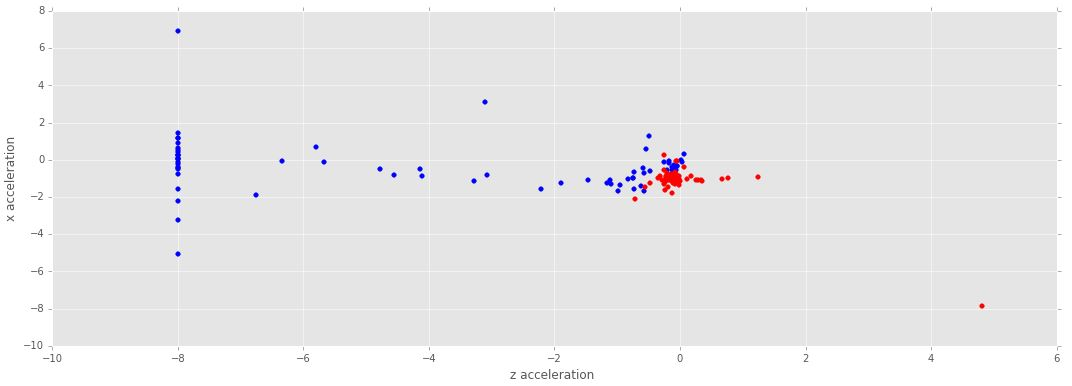
\includegraphics[width=0.9\textwidth]{PE4/xzplot2.JPG}
\caption{Distribution of data points labeled as collision (blue) or no collision (red)}
\label{fig:xyscatter}
\end{figure}

\section{Solution strategy}
\label{sec:Solution strategy}
Combining the knowledge about the sensor data from the previous section and the objective as described in chapter \ref{ch:Introduction}, this chapter will narrow down on a specific problem type and solution strategy. In the process, the limitations described in Chapter \ref{ch:Introduction} have to be considered. \\
A corpus of sensor data was collected as described above and labelled according to the event of a collision or no collision. In chapter \ref{ch:Introduction}  the necessity of using the Apache Spark library module ``MLLib'' is constituted.
\\ 
Having a set of labeled sensor data allows for a supervised machine learning approach.  Furthermore the existence of concrete data points which represent the state of the Sensorboard at a given time makes it possible to base the recognition of collisions solely on single data points. The recognition of collisions can then in turn be formulated as the problem of deciding weather a given data point corresponds to a collision or no collision. A problem of this kind can be solved by binary classification. \\
Having specified the solution method to a binary classification approach, specific algorithms can be considered. For the specific task of supervised binary classification the following algorithms are supported by the MLLib module:

\begin{itemize}
\item Linear SVM
\item Logistic regression
\item Decision tree
\item Random forest
\item Gradient-boosted trees
\item Naive Bayes
\end{itemize}

Only the possible algorithms mentioned here will be parameterized and trained on the  collected data in chapter \ref{ch:Algorithm configuration}.   \\

To assess the performance of resulting models a clear metric will be used for comparison. This metric has to represent the unequal importance of detecting a collision and preventing false alarms. As mentioned in chapter \ref{ch:Introduction} the act of detecting a collision that actually happened (\emph{true positives}) is more important than preventing the detection of a collision that didn't happen (\emph{false positives}). In a classification setting the effectiveness in detecting collision that actually happened is described by recall. The effectiveness of preventing the detection of collision that didn't happen is described by precision. The metric that will be used to represent the unequal relationship between precision and recall is a\emph{ f\textsubscript{2}-score}. This metric puts more weight on the recall of a model. This way a later evaluation of trained classifiers can be done based on one correctly weighted metric.